\chapter{Motivation for Convolution}

Convolution introduces three key principles: \textit{sparse interactions}, \textit{parameter sharing} and \textit{equivariance to translation} \cite{goodfellow2016deep}.  

\section{Sparse interactions}

In a traditional neural network layer, every output unit interacts with every input unit.  
For high-dimensional data, such as images, this leads to an extremely large number of parameters.  
Convolution addresses this by connecting each output only to a local neighborhood of the input, known as its \textit{receptive field}.

If the kernel has size $k \times k$, then each output depends on only $k^2$ inputs, rather than the entire input dimension. It is often possible to obtain very good performance on a ML task while keeping $k$ several orders of magnitude smaller than the inputs.

\clearpage

This sparsity not only reduces the number of parameters, but also encodes the prior knowledge that local groups of variables are often more strongly correlated than distant ones.  

\begin{figure}[H]
    \centering
    \begin{minipage}{0.45\textwidth}
        \centering
        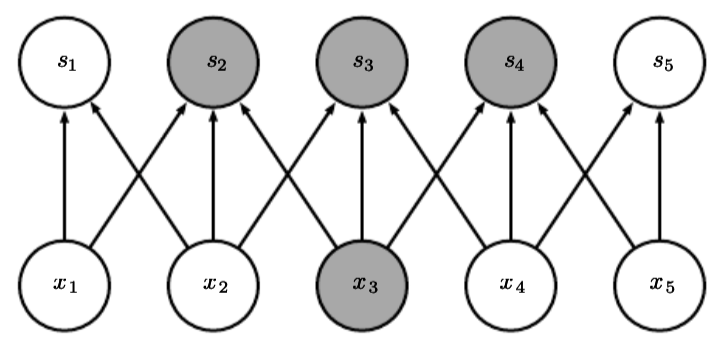
\includegraphics[width=\linewidth]{Images/Chapters/sparsity_1.png}
    \end{minipage}
    \hfill
    \begin{minipage}{0.45\textwidth}
        \centering
        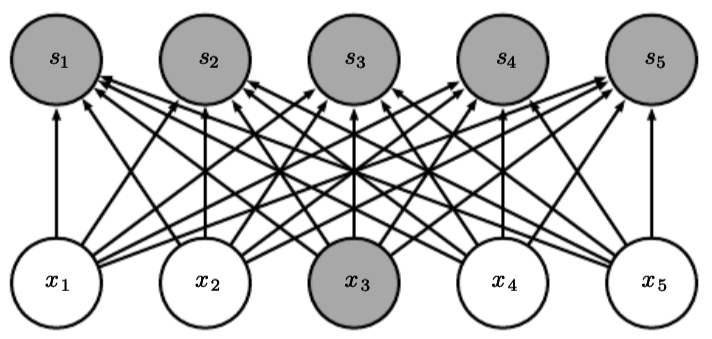
\includegraphics[width=\linewidth]{Images/Chapters/sparsity_2.png}
    \end{minipage}
    \caption{Sparse connectivity: when \textit{s} is formed by convolution (left), and when \textit{s} is formed by matrix multiplication (right).}
    \label{fig:sparsity}
\end{figure}



In a deep convolutional network, stacking multiple convolutional layers allows units in deeper layers to have larger receptive fields, enabling them to capture more abstract and global features by efficiently constructing complex interactions from simple local ones.

\begin{figure}[H]
    \centering
    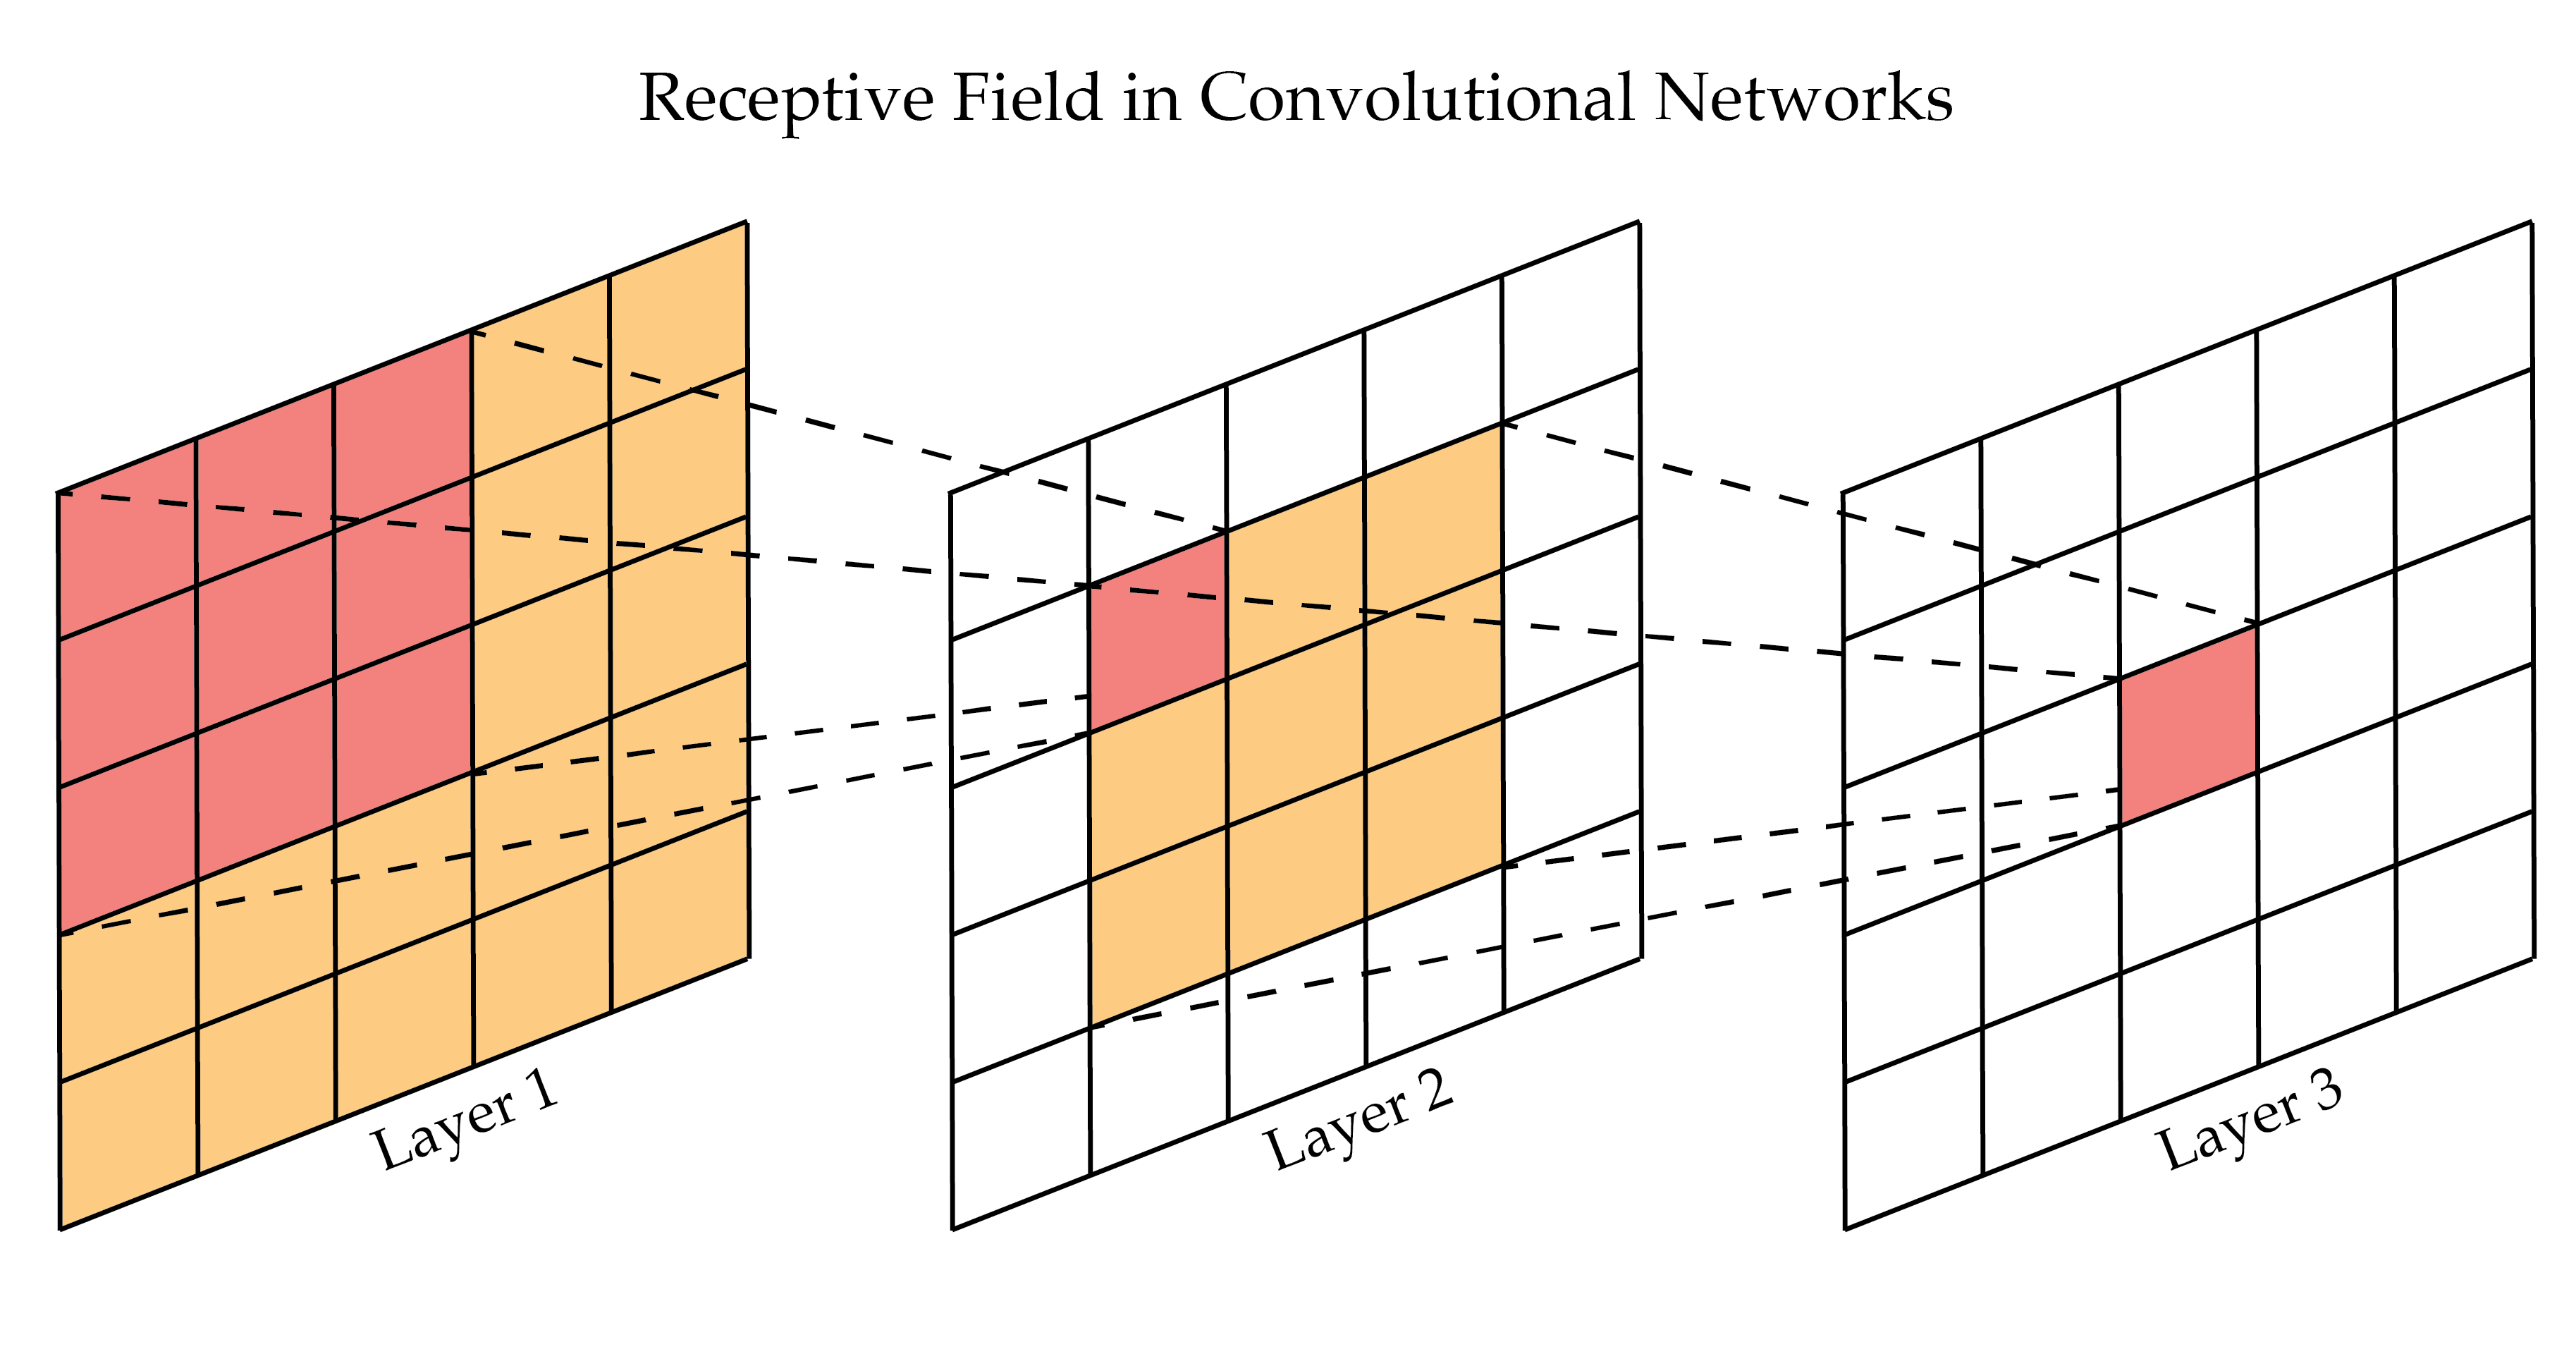
\includegraphics[width=0.5\linewidth]{Images/Chapters/receptive_fields.png}
    \caption{Visualization of growing receptive fields across CNN layers.}
    \label{fig:receptive_fields}
\end{figure}

\section{Parameter sharing}

Another advantage of convolution is that the same kernel is applied across all spatial locations.  
We can say that the network has \textit{tied weights}, because the values of the weight are the same everywhere. This means that instead of learning a separate set of weights for each location, the model learns only one kernel that is reused.  

For example, a kernel that detects vertical edges will detect them anywhere in the image. This does not affect the runtime of forward propagation, still $O(k\times n)$ where $k$ is the kernel size and the input is $m\times n$.

\clearpage

This greatly reduces the number of learnable parameters and improves generalization, since the same features are useful at multiple positions.

\begin{figure}[H]
    \centering
    \begin{minipage}{0.45\textwidth}
        \centering
        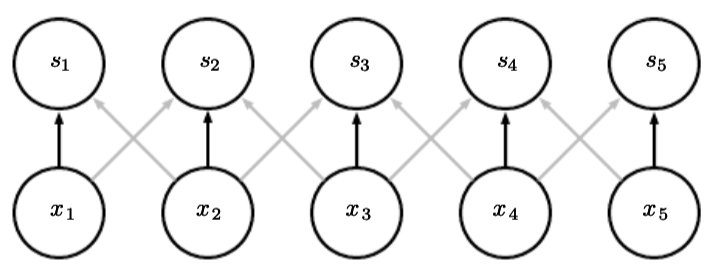
\includegraphics[width=\linewidth]{Images/Chapters/param_sharing2.png}
    \end{minipage}
    \hfill
    \begin{minipage}{0.45\textwidth}
        \centering
        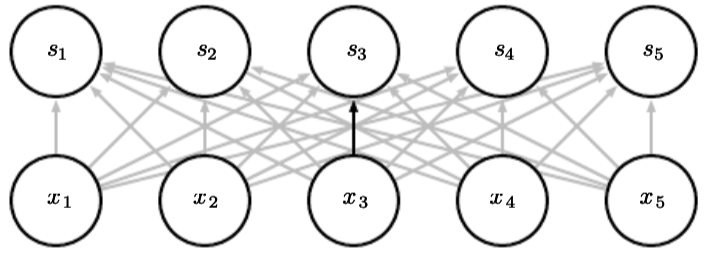
\includegraphics[width=\linewidth]{Images/Chapters/param_sharing1.png}
    \end{minipage}
    \caption{Parameter sharing: because of parameter sharing, the single parameter is used everywhere (left); in the other hand the parameter is used only once (right).}
    \label{fig:param_sharing}
\end{figure}

\section{Equivariance to translation}

The already discussed parameter sharing causes in convolution a property called \textit{equivariance} to translation.  
Formally, a function $f$ is equivariant to an operation $T$ if, applying $T$ to the input and then $f$, gives the same result as applying $f$ first and then $T$ to the output.  

Convolution satisfies this property with respect to translations:  
\[
(K * I)(x + \Delta) = T_{\Delta} \big( (K * I)(x) \big),
\]
where $T_{\Delta}$ denotes a translation by $\Delta$.  

This means that if the input image is shifted, the output feature map shifts in the same way. In images, convolution produces a 2-D feature map where detected patterns shift consistently with the input, enabling parameter sharing across locations. This is useful for features like edges, which appear throughout an image, though in some cases, such as face recognition, different regions may require learning distinct features. 